%  Introduction.tex
%  Document created by seblovett on seblovett-Ubuntu
%  Date created: Tue 01 Apr 2014 19:50:43 BST
%  <+Last Edited: Fri 04 Apr 2014 15:55:01 BST by hl13g10 on octopus +>

\section{Introduction}\label{sect:intro}
%\todo[inline]{Introduction to do}
%State the objectives of the assignment. Summarise briefly your preparation work,  your experimental work,, and results achieved. Specifically, state which parts of the assignment were delivered according to the requirements and summarise any extensions to the basic specification you have carried out with references to the sections.  ( approx. 0.5 page).

This assignment is to design and test a processor capable of executing an affine transform of a vector. 
The processor should be optimised in terms of size, with no performance requirements. 
The cost function, seen in equation~\eqref{eq:cost}, should be minimised. 
The data is given in bytes and must be read from the switches and the result should be displayed on the LEDs. 
A handshaking protocol is also defined and must be followed. 
A processor is defined as having a distinct control, datapath and memory with an instruction set that is executed. 

\begin{equation}\label{eq:cost}
\mbox{Cost} = \mbox{ Number of Logic Elements} + 30 \times \mbox{Kbits of RAM}
\end{equation}

A number of designs and approaches were investigated, including register-register and single cycle designs.
The final design is a register-accumulator, multi-cycle processor which utilises embedded multipliers and SRAM available on the FPGA. 
It is able to conduct the affine transform using data set 2 (see equation \ref{eq:affinedata2}) and satisfies the handshaking protocols. 

\begin{equation}\label{eq:affinedata2}
\begin{bmatrix}
x_2 \\
y_2 
\end{bmatrix}
=
\begin{bmatrix}
0.5 & -0.875 \\
-0.875 & 0.75 
\end{bmatrix}
\begin{bmatrix}
x_1 \\
y_1
\end{bmatrix}
+
\begin{bmatrix}
5 \\
12
\end{bmatrix}
\end{equation}


Figure \ref{fig:arch} shows the architecture of the processor, excluding the control and control signals.

\begin{figure}
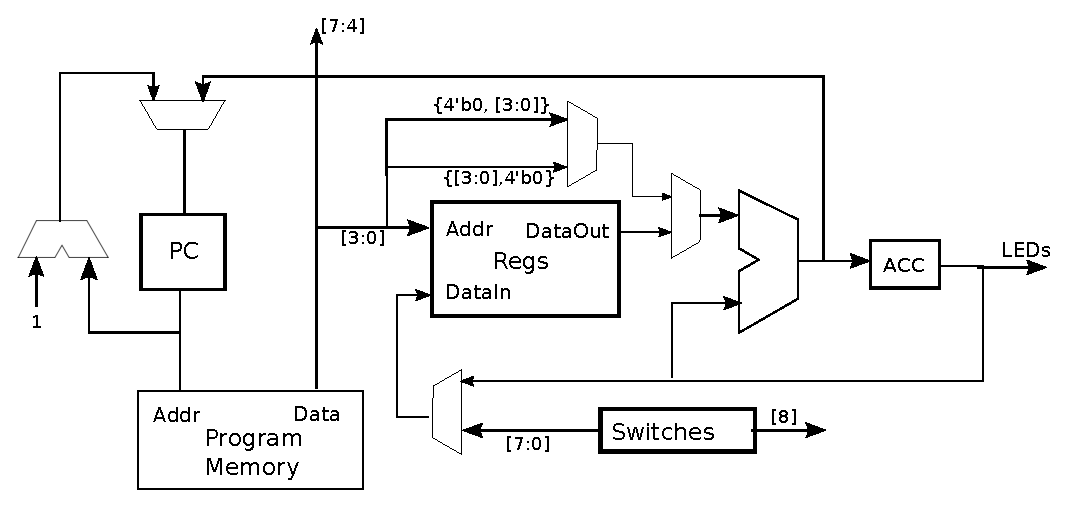
\includegraphics[width=\textwidth]{Figures/architecture.eps}
\caption{Block Diagram of the architecture. Control unit and signals have been omitted for clarity.}
\label{fig:arch}
\end{figure}

Each module of the processor is documented in this report, with discussion on the design, test and synthesis of the code. 
Additional extras are also discussed, including a simple assembler (see section \ref{sect:prog} and extra logic added for debugging and the demonstration (see section \ref{sect:de0}.
